\documentclass[a4paper,11pt]{article}
\usepackage[T1]{fontenc}
\usepackage[utf8]{inputenc}
\usepackage[slovene]{babel}
\usepackage[margin=2.5cm]{geometry}
\usepackage{amsmath,amssymb}
\usepackage{graphicx}
\usepackage{enumitem}
\usepackage{tabularx}
\usepackage{ragged2e}
\usepackage{tikz}
\usepackage{xcolor}
\usepackage{lmodern}

\newcommand{\RR}{\mathbb{R}}

\newenvironment{ide}{%
  \par\medskip\noindent\textbf{Ideja.}\itshape\ }{\par\medskip}
\newenvironment{komentar}{%
  \par\medskip\noindent\textbf{Komentar.}\itshape\ }{\par\medskip}
\newenvironment{primer}{%
  \par\medskip\noindent\textbf{Primer.}\itshape\ }{\par\medskip}

\begin{document}

\title{Pregled snovi: Vektorji}
\author{}
\date{}
\maketitle

\tableofcontents
\newpage
\section{1. ura: Osnove}
\begin{tabularx}{\textwidth}{|>{\bfseries\RaggedRight}p{2.7cm}|X|}
\hline
Oblika & Frontalna, delo v skupinah \\ \hline
Pripomočki & Tabla, kreda, ravnilo, (avtomobilčki) \\ \hline
Učni cilji & Osvojiji pojem vektorja \\ \hline
Predznanje & Mogoče iz fizike \\ \hline

\end{tabularx}
\\

\begin{ide}
    Za uvod se lahko igramo z avtomobilčki (igračami): Dijaki označijo začetno točko avtomobilčka, nato pa ga večkrat porinejo, v različne smeri in z različno močjo. Po vsakem premiku narišejo pot, kje je avtomobilček vozil, ter označijo smer, v katero se je avtomobilček po tej poti premikal. Tako dobimo en kup različnih vektorjev. Lahko jih pustiš za konec ure, da bodo lahko izmerili kateri vektorji so enako dolgi, enako usmerjeni, nasprotno usmerjeni, itd.
\end{ide}

Vektorje povežem z njihovim pojmovanjem v fiziki (ponazarjajo kam se nekaj premika).
\textbf{DEFINICIJA:} Vektor je množica usmerjenih daljic, ki imajo isto:
\begin{itemize}
    \item smer (smer je določena s premico nosilko vektorja)
    \item usmerjenost (kam kaže puščica)
    \item velikost (dolžino vektorja- označimo jo z $|\vec{AB}|=d(A,B)$)
\end{itemize}
Vektorja, ki ležita na vzporednih nosilkah imata enako smer. \\
Nato narišemo vektor in pokomentiramo označevanje vektorjev (z malimi črkami ali pa velikimi tiskanimi, ki ponazarjajo začetno in končno točko)\\
Vektorja sta enaka, če sta vzporedna, enako velika in enako usmerjena. (podam primer)\\
Z vzporednim premikom vektor ohranjamo.\\
\textbf{Ničelni vektor} je vektor, ki ima dolžino nič: $\vec{AA}=\vec{0}$\\
\textbf{Enotski vektor} je vektor, ki ima dolžino ena: $|\vec{e}|=1$\\
\textbf{Nasprotni vektor} vektorja $\vec{AB}$, je vektor, ki je vzporeden vektorju $\vec{AB}$, ima enako dolžino kot $\vec{AB}$ in je nasprotno usmerjen kot $\vec{AB}$. Zapis: $-\vec{AB}$
\begin{komentar}
    $\vec{AB}=-\vec{BA}$
\end{komentar}
Na tablo narišem vse zgoraj omenjene vektorje.\\
Nato narišemo enostavnejše geometrijske like (pravokotnik, kvadrat, pravilni šestkotnik) in se pogovarjamo, kateri vektorji so enaki, kateri nasprotni, kateri imajo enako dolžino, kateri so ničelni vektorji, kateri so enotski.\\

%%%%%%%%%%%%%%%%%%%%%%%%%%%%%%%%%%%%%%%%%%%%%%%%%%%%%%%%%%%%%%%%%%%%%%%%%%%%%%%%%%%%%%%%%%%%%%%%%%%%%%%%%%%%%%%%%%%%%%%%%%%%%%%%%%%%%%%%%%%%%%%%%%%%%%%%%%%%%%%%%

\newpage \section{2. ura: Seštevanje vektorjev}
\begin{tabularx}{\textwidth}{|>{\bfseries\RaggedRight}p{2.7cm}|X|}
\hline
Oblika & Frontalna \\ \hline
Pripomočki & Tabla, kreda, ravnilo \\ \hline
Učni cilji & Narišejo vektorje in grafično seštevajo  \\ \hline
Predznanje &  \\ \hline

\end{tabularx}
\\

Vsota/ razlika vektorjev je vektor.\\
\\
\textbf{SEŠTEVANJE}\\
Dva načina, kako geometrijsko seštevamo vektorje:
\begin{enumerate}
    \item \textbf{paralelogramsko pravilo}:\\
    vektorja pomaknemo tako, da se začneta v isti točki. Narišemo paralelogram, ki ima ta dva vektorja kot stranici. Diagonala, ki se začne v izhodiščih teh dveh vektorjev, je vsota danih vektorjev. 
    \item \textbf{trikotniško pravilo}:\\
    Razložim, da izhaja iz paralelogramskega pravila. Začetek enega vektorja premaknemo v konec drugega vektorja. Vektor, ki povezuje začetek prvega vektorja in konec drugega vektorja, je vsota danih vektorjev.
\end{enumerate}
Nato na enostavnih likih (pravokotnik, pravilni šestkotnik) naredimo par primerov seštevanja vektorjev.\\
Pogledamo tudi primer, kaj se zgodi, ko v pravilnem šestkotniku seštejemo vse vektorje ($\vec{AB}+\vec{BC}+\vec{CD}+\vec{DE}+\vec{EF}+\vec{FA}$). Zakaj se to zgodi? Opazimo, da v primeru nastopa seštevanje nasprotnih vektorjev.\\
S pomočjo geometrijske predstave razmislimo katere lastnosti ima seštevanje:
\begin{itemize}
    \item komutativnost (zakon o zamenjavi): $\vec{a}+\vec{b}=\vec{b}+\vec{a}$
    \item asociativnost (zakon o združevanju): $(\vec{a}+\vec{b})+\vec{c}=\vec{a}+(\vec{b}+\vec{c})$
    \item nevtralni element za seštevanje: $\vec{a}+\vec{0}=\vec{a}$
    \item $\vec{a}+(-\vec{a})=\vec{0}$
    \item $-(-\vec{a})=\vec{a}$
\end{itemize}
%%%%%%%%%%%%%%%%%%%%%%%%%%%%%%%%%%%%%%%%%%%%%%%%%%%%%%%%%%%%%%%%%%%%%%%%%%%%%%%%%%%%%%%%%%%%%%%%%%%%%%%%%%%%%%%%%%%%%%%%%%%%%%%%%%%%%%%%%%%%%%%%%%%%%%%%%%%%%%%%%%
\newpage \section{3. ura: Odštevanje vektorjev}
\begin{tabularx}{\textwidth}{|>{\bfseries\RaggedRight}p{2.7cm}|X|}
\hline
Oblika & Frontalna \\ \hline
Pripomočki & Tabla, kreda, ravnilo \\ \hline
Učni cilji & Grafično odštevajo vektorje \\ \hline
Predznanje & Seštevanje vektorjev \\ \hline

\end{tabularx}
\\
\textbf{ODŠTEVANJE}\\
Odštevanje definiramo kot prištevanje nasprotnih vektorjev: $\vec{a}-\vec{b}=\vec{a}+(-\vec{b})$.\\
Na tablo narišem primer, s katerim po korakih utemeljim zgornjo trditev (narišem dva vektorja $\vec{a}$ in $\vec{b}$, nato vektorju $\vec{b}$ narišem njemu nasprotni vektor, ga premaknem tako, da lahko uporabim trikotniško pravilo za seštevanje vektorjev).\\
Nato na enostavnih likih (pravokotnik, pravilni šestkotnik) naredimo par primerov odštevanja vektorjev.\\


%%%%%%%%%%%%%%%%%%%%%%%%%%%%%%%%%%%%%%%%%%%%%%%%%%%%%%%%%%%%%%%%%%%%%%%%%%%%%%%%%%%%%%%%%%%%%%%%%%%%%%%%%%%%%%%%%%%%%%%%%%%%%%%%%%%%%%%%%%%%%%%%%%%%%%%%%%%%%%%%%%
\newpage \section{4. ura: Množenje vektorja s številom/ skalarjem}
\begin{tabularx}{\textwidth}{|>{\bfseries\RaggedRight}p{2.7cm}|X|}
\hline
Oblika & Frontalna \\ \hline
Pripomočki & Tabla, kreda, ravnilo \\ \hline
Učni cilji & Množijo vektorje s skalarjem \\ \hline
Predznanje & Seštevanje vektorjev \\ \hline

\end{tabularx}
\\

Za uvod v  to temo najprej narišemo nek vektor $\vec{a}$. Kako naj bi izgledal vektor $2\vec{a}=\vec{a}+\vec{a}$?  Kaj pa vektor $-2\vec{a}$? Kaj pa vektor $\frac{1}{2}\vec{a}$?\\
\begin{ide}
    Razmislek lahko povežemo z avtomobilčki iz prejšnje ure: nekdo je porinil avtomobilček in pri tem s puščico označil njegovo pot. Nato je prišel drugi sošolec in iz iste točke porinil avtomobilček 2x močneje. Kako bo izgledala puščica, ki jo bo ob tem narisal?
\end{ide}
Pri množenju vektorja s skalarjem $m$ dobimo vektor.\\

$m\cdot\vec{a}$; $m\in\RR$, $m\not=0$
\begin{itemize}
    \item $m\vec{a}$ je vzporeden vektorju $\vec{a}$ (smer se ohranja)
    \item $|m\vec{a}|=|m||\vec{a}|$
    \item $m>0\Rightarrow$ usmerjenost enaka, $m<0\Rightarrow$ usmerjenost nasprotna
    \item $|m|>1\Rightarrow$ vektor bo daljši, $|m|<1\Rightarrow$ vektor bo krajši
\end{itemize}
Natančneje definirajmo enotski vektor: za začetni primer narišimo vektor $\vec{a}$ ki ima dolžino $|\vec{a}|=3$. Na tem vektorju označimo enotski vektor $\vec{e_a}$. Na danem primeru pojasnim naslednjo enačbo: $$\vec{e_a}=\frac{1}{|\vec{a}|}\vec{a}$$.\\
\textbf{LASTNOSTI MNOŽENJA VEKTORJA S SKALARJEM:}
\begin{itemize}
    \item asociativnost: $m(n\vec{a})=(mn)\vec{a}$
    \item distributivnost v vektorskem faktorju: $m(\vec{a}+\vec{b})=m\vec{a}+m\vec{b}$
    \item distributivnost v skalarnem faktorju: $(m+n)\vec{a}=m\vec{a}+n\vec{a}$
\end{itemize}
Sledijo vaje. Vaje naj vključujejo tudi naloge, s katerimi utrdimo zgornje lastnosti množenja vektorja s skalarjem.\\
\begin{primer}
    Dana sta vektorja $\vec{a}$ in $\vec{b}$. Nariši vektor $2\vec{a}-3\vec{b}$.
\end{primer}
\begin{primer}
    Dana sta vektorja $\vec{u}=\vec{a}-\frac{1}{2}\vec{b}$ in $\vec{v}=\frac{1}{2}\vec{a}+\vec{b}$. Z $\vec{a}$ in $\vec{b}$ izrazi vektor $3\vec{u}+2\vec{v}-4(\vec{u}-\frac{1}{2}\vec{b})$.
\end{primer}
Na tem mestu lahko rešimo tudi enostavnejšo vektorsko enačbo.
\begin{primer}
    Reši vektorjsko enačbo $3(\vec{x}+2\vec{a}-\vec{b})=\vec{b}+5\vec{a}+\frac{1}{2}(\vec{x}-2\vec{c})$.
\end{primer}
\begin{primer}
    V trikotniku $\triangle ABC$ točka $D$ deli stranico $AC$ v razmerju $|AD|:|DC|=2:1$, točka $E$ pa razpolovi daljico $DB$. Označimo $\vec{a}=\vec{AB}$ in $\vec{b}=\vec{AC}$. Izrazi naslednje vektorje z vektorjema $\vec{a}$ in $\vec{b}$:  $\vec{DE}=?$, $\vec{AE}=?$, $\vec{CE}=?$.
\end{primer}

%%%%%%%%%%%%%%%%%%%%%%%%%%%%%%%%%%%%%%%%%%%%%%%%%%%%%%%%%%%%%%%%%%%%%%%%%%%%%%%%%%%%%%%%%%%%%%%%%%%%%%%%%%%%%%%%%%%%%%%%%%%%%%%%%%%%%%%%%%%
\newpage
\section{5. ura: Dodatna ura}
\begin{tabularx}{\textwidth}{|>{\bfseries\RaggedRight}p{2.7cm}|X|}
\hline
Oblika & Vaje pred tablo \\ \hline
Pripomočki & Tabla, kreda, vaje \\ \hline
Učni cilji & Grafično seštevajo, odštevajo in množijo vektorje s skalarjem. Rešujejo enostavnejše vektorske enačbe. \\ \hline
Predznanje & Seštevanje, odštevanje in množenje vektorja s skalarjem \\ \hline

\end{tabularx}
\\

Na geometrijskih likih rišemo vektorje, ki so vsota, razlika ali pa večkratnik nekih drugih vektorjev.\\

Primerna naloga je tudi:
\begin{primer}
    Reši vektorsko enačbo: $$3(\vec{x}+2\vec{a}-\vec{b})=\vec{b}+5\vec{a}+\frac{1}{2}(\vec{x}-2\vec{c})$$
\end{primer}
%%%%%%%%%%%%%%%%%%%%%%%%%%%%%%%%%%%%%%%%%%%%%%%%%%%%%%%%%%%%%%%%%%%%%%%%%%%%%%%%%%%%%%%%%%%%%%%%%%%%%%%%%%%%%%%%%%%%%%%%%%%%%%%%%%%%%%%%%%%%%%%%%%%%%%%%%%%%%%%%%%%
\newpage \section{6. ura: Odvisni in neodvisni vektorji v ravnini, baza ravnine}
\begin{tabularx}{\textwidth}{|>{\bfseries\RaggedRight}p{2.7cm}|X|}
\hline
Oblika & Frontalna, diskusija \\ \hline
Pripomočki & Tabla, kreda, (avtomobilčki, puščice) \\ \hline
Učni cilji & Presodijo kolinearnost in koplanarnost vektorjev \\ \hline
Predznanje & Množenje vektoja s skalarjem, seštevanje vektorjev \\ \hline

\end{tabularx}
\\

\noindent Najprej definirajmo pojme kolinearnost, koplanarnost in nekoplanarnost, da ne bo pozneje prišlo do zmede.\\
Vektorja sta \textbf{kolinearna}, če sta vzporedna ali če eden izmed njiju ničelni vektor. Sicer sta nekolinearna. Opomba: kolinearnih je lahko tudi več vektorjev hkrati.
Na tablo narišem vektor $\vec{a}$ in vektor $\vec{b}$, ki leži nekje na vektorju $\vec{a}$. Zapišemo lahko $\vec{a}=m\vec{b}$.\\
Vektorjem, ki ležijo v isti ravnini, rečemo, da so \textbf{koplanarni}. \\
Če ne ležijo v isti ravnini so \textbf{nekoplanarni}.
\begin{ide}
    Profesor lahko pred začetkom ure nalepi različne puščice po razredu. Z dijaki nato ugotavljamo kateri izmed teh vektorjev (puščic) so kolinearni (ležijo na vzporednih robovih miz npr.), kateri koplanarni (ležijo na istem zidu, na tleh,..) in kateri nekoplanarni. Ugotovimo, da so vsi vektorji skupaj del istega prostora, ker ne ležijo vsi na isti ravnini so nekoplanarni.
\end{ide}


Nato začnemo z enostavnim primerom: 
\begin{primer}
    Poenostavi predpis za vektor $\vec{u}$: $\qquad \vec{u}=7\vec{a}-5\vec{b}-2(\vec{a}-\vec{b})$
\end{primer}
\noindent Rezultat bomo imenovali linearna kombinacija (vektorjev $\vec{a}$ in $\vec{b}$).\\
Formalno: Zapis $k\vec{a}+l\vec{b}$ imenujemo \textbf{linearna kombinacija} vektorjev $\vec{a}$ in $\vec{b}$. Podam še druge primere, da pokažem, da linearna kombinacija ni nujno sestavljena iz natanko dveh vektorjev.\\
Vrnimo se nazaj na linearno kombinacijo dveh vektorjev:
Vektor $k\vec{a}+l\vec{b}$ grafično predstavim, tako da narišem vektor $\vec{a}$, vektor $\vec{b}$, nato vektor $k\vec{a}$, $l\vec{b}$ in nato $k\vec{a}+l\vec{b}$.\\
Dva poljubna neničelna linearno neodvisna vektorja $\vec{a}$ in $\vec{b}$ tvorita \textbf{bazo ravnine}. To pomeni, da lahko vsak vektor v tej ravnini zapišemo na en sam način -- kot linearno kombinacijo teh dveh vektorjev.\\ 
\begin{ide}
    Dijakom lahko tole jasneje razložim tako, da imam s seboj avtomobilčke (igrače), ki se lahko premikajo po tabli samo po eni premici. Če imam dva avtomobilčka, nanju zavežem vrvico na kateri je kreda 
    (ali pa nanju pritrdim konca šestila da se ni potrebno truditi z risanjem ravne črte s pomočjo vrvice -- šestilo se upogiba in zna z oddaljevanjem avtkov narisati ravno premico (preveri če deluje)).
     S premiki teh dveh avtomobilčkov lahko s privezano kredo narišem poljuben vektor v ravnini. Če imam samo en avtomobilček, lahko narišem samo vektorje, ki ležijo na premici po kateri se ta avtomobilček premika.
      Če imam tri avtomobilčke, lahko prav tako narišem vse vektorje, vendar rečemo, da ti trije vektorji niso baza, saj za bazo vedno vzamemo najmanjše možno število avtomobilčkov ki jih potrebujemo, da narišemo vse vektorje v ravnini. Razmislimo, kaj moramo narediti, da bi lahko narisali vektor, ki ne leži na tabli.
\end{ide}
Bazo prostora tvorijo trije neničelni vektorji, ki ne ležijo na isti ravnini (v nadaljevanju trije linearno neodvisni vektorji). Vsak vektor v prostoru lahko na enoličen način izrazimo z linearno kombinacijo teh treh vektorjev: $$\vec{v}=k\vec{a}+l\vec{b}+m\vec{c}; k,l,m\in\RR$$.\\

Če lahko en vektor zapišemo s pomočjo drugih vektorjev (linearna kombinacija) pravimo, da so \textbf{linearno odvisni}.\\
Če vektorja ne moremo zapisati s pomočjo drugih vektorjev, pravimo, da so \textbf{linearno neodvisni}. (To lahko utrdimo na primeru avtomobilčkov.) Drugače povedano: vektorja $\vec{a}$ in $\vec{b}$ sta linearno neodvisna, če velja: $$k\vec{a}+l\vec{b}=\vec{0}\Rightarrow k=0\text{ in }l=0;\qquad k,l\in\RR$$

%%%%%%%%%%%%%%%%%%%%%%%%%%%%%%%%%%%%%%%%%%%%%%%%%%%%%%%%%%%%%%%%%%%%%%%%%%%%%%%%%%%%%%%%%%%%%%%%%%%%%%%%%%%%%%%%%%%%%%%%%%%%%%%%%%%%%%%%%%%%%%%%%%%%%%%%%%%%%%%%%%%%
\newpage \section{7. ura: Odvisni in neodvisni vektorji v prostoru, baza prostora}
\begin{tabularx}{\textwidth}{|>{\bfseries\RaggedRight}p{2.7cm}|X|}
\hline
Oblika & Frontalna, vaje pred tablo \\ \hline
Pripomočki & Tabla, kreda \\ \hline
Učni cilji &  Presodijo linearno neodvisnost vektorjev\\ \hline
Predznanje & Znanje  prejšnje ure \\ \hline

\end{tabularx}
\\

Ker smo v zadnjih dveh urah spoznali veliko novih pojmov, naredimo povzetek vseh pojmov, da si jih bodo lažje zapomnili in manj mešali med seboj:\\
\textbf{Kolinearni vektorji}, so tisti, ki so vzporedni, torej jih lahko premaknemo tako, da ležijo na isti premici. \textbf{Koplanarni vektorji} ležijo na isti ravnini. \textbf{Nekoplanarni vektorji} pa so del (istega) prostora.\\
\textbf{Baza ravnine} sta dva linearno neodvisna vektorja, \textbf{baza prostora} pa trije linearno neodvisni vektorji.\\
\textbf{Linearno odvisni} vektorji so tisti, ki jih lahko zapišemo z uporabo drugih vektorjev, \textbf{linearno neodvisni} pa tisti, ki jih ne moremo zapisati z uporabo drugih vektorjev.\\
\\

Sledijo vaje, ki vključujejo naloge, s katerimi utrdimo zgornje pojme. Na začetku naloge se vprašamo, kaj je baza ravnine, med nalogo pa kateri vektorji so linearno (ne)odvisni, kaj je linearna kombinacija, itd. Začnemo na lažjih primerih, npr. na enostavnih likih in geometrijskih telesih. Pri geometrijskih telesih si lahko pomagamo s 3D modeli geometrijskih teles.\\
Ostali primeri:
\begin{primer}
    naj vektorja $\vec{a}$ in $\vec{b}$ tvorita bazo ravnine. Določi vrednosti $m$ in $n$, da velja: $(n-2)(\vec{a}+\vec{b})=3(m\vec{a}+\vec{b})$.
\end{primer}
\begin{komentar}
    Rešitev: $m=1, n=5$
\end{komentar}
\begin{primer}
    Dokaži, da v trikotniku težišče težiščnice tretjini.
\end{primer}
\begin{komentar}
    Postopek: izberemo bazo, zapišemo vektor $\vec{AT}$ na dva načina, enačimo dobljena izraza in tako pridemo do rešitve.
\end{komentar}
\begin{primer}
    Imamo paralelogram $ABCD$. Točka $P$ leži na daljici $BC$ tako, da velja $|BP|:|PC|=1:3$, točka $E$ pa leži na preseku daljic $AP$ in $BD$. Izračunaj, v kakšnem razmerju $E$ deli $BD$.
\end{primer}
\begin{komentar}
    Rešitev: $|BE|:|ED|=1:4$
\end{komentar}

%%%%%%%%%%%%%%%%%%%%%%%%%%%%%%%%%%%%%%%%%%%%%%%%%%%%%%%%%%%%%%%%%%%%%%%%%%%%%%%%%%%%%%%%%%%%%%%%%%%%%%%%%%%%%%%%%%%%%%%%%%%%%%%%%%%%%%%%%%%%%%%%%%%%%%%%%%%%%%%%%%%%%%%%%%%%%
\newpage \section{8. ura: Vaje}
\begin{tabularx}{\textwidth}{|>{\bfseries\RaggedRight}p{2.7cm}|X|}
\hline
Oblika &  Individualno delo \\ \hline
Pripomočki & Delovni listi \\ \hline
Učni cilji & Utrdijo snov o vektorjih \\ \hline
Predznanje & Dosedanje znanje o vektorjih \\ \hline

\end{tabularx}
\\

Ponovimo celotno snov o vektorjih: od najlažje k težjim nalogam.\\

\begin{primer}
    V pravilnem osemkotniku $ABCDEFGH$:
    \begin{itemize}
        \item določi vse pare enakih vektorjev,
        \item določi 4 pare nasprotnih vektorjev,
        \item določi 4 vektorje enake dolžine kot $\vec{AC}$, 
        \item določi vse ničelne vektorje,
        \item poišči vse vektorje, ki imajo enako smer kot $\vec{CD}$.
    \end{itemize}
\end{primer}
\begin{primer}
    Dani so vektorji:
    \[     \vec{a}=\vec{AB}, \qquad \vec{b}=\vec{CD}, \qquad \vec{c}=\vec{BA}.     \]
    \begin{enumerate}
        \item Kateri vektor je nasprotni vektor vektorja $\vec{a}$?
        \item Kdaj velja $\vec{a}=\vec{b}$?
        \item Ali sta lahko $\vec{a}$ in $\vec{c}$ enaka? Utemelji.
    \end{enumerate}
\end{primer}
\begin{primer}
    Nariši:
    \begin{enumerate}
        \item vektor dolžine $4$,
        \item enotski vektor,
        \item ničelni vektor,
        \item nasprotni vektor podanega vektorja $\vec{u}$.
    \end{enumerate}
\end{primer}
\begin{primer}
    S trikotniškim pravilom izračunaj:
    $\vec{AB}+\vec{BC},
    \vec{CD}+\vec{DA}.$
    Kaj opaziš?
\end{primer}
\begin{primer}
    V paralelogramu $ABCD$ izrazi z enim vektorjem:
    \[     \vec{AB}+\vec{BC},    \]
    \[    \vec{AB}+\vec{AD},    \]
    \[    \vec{AC}-\vec{AD}.    \]
\end{primer}
\begin{primer}
    Poenostavi: %??dej še kej ulomku vmes da bo težje
    \[    \vec{a}+\vec{b}-\vec{a},    \]
    \[    2\vec{a}-\vec{a}+\vec{b},    \]
    \[    \vec{a}+(-\vec{a})+\vec{b}.    \]
\end{primer}
\begin{primer}
    Nariši vektor: %?? dej še kej ulomku da bo težje
    \[    2\vec{a}+\vec{b}-\vec{c}.    \]
\end{primer}
\begin{primer}
    Nariši:
    \[    2\vec{a}, \qquad -\vec{a}, \qquad -2\vec{a}, \qquad \frac12\vec{a}.    \]
    Za vsak vektor povej:
    \begin{itemize}
        \item ali ima enako smer,
        \item ali ima enako usmerjenost,
        \item ali je daljši ali krajši od $\vec{a}$.
    \end{itemize}
\end{primer}
\begin{primer}
    Če je $|\vec{a}|=5$, izračunaj:
    \[    |2\vec{a}|, \qquad    \left|-\frac12\vec{a}\right|, \qquad    |3\vec{a}|.    \]
\end{primer}
\begin{primer}
    Poenostavi izraz: %?? naredi težje,...
    \[    3(\vec{a}+\vec{b})-2\vec{a}+\vec{b}.    \]
\end{primer}
\begin{primer}
    Dana sta:
    \[    \vec{u}=2\vec{a}-\vec{b}, \qquad    \vec{v}=\vec{a}+3\vec{b}.    \]
    Izrazi vektor:
    \[    2\vec{u}-\vec{v}    \]    z vektorjema $\vec{a}$ in $\vec{b}$.
\end{primer}
\begin{primer}
    Reši vektorsko enačbo:
    \[    2(\vec{x}+\vec{a})=3\vec{b}+\vec{x}.   \]
\end{primer}
\begin{primer}
    Reši vektorsko enačbo:
    \[    4(\vec{x}-\vec{a})=2(\vec{x}+\vec{b}).    \]
\end{primer}
\begin{primer}
    Naj bo $|\vec{a}|=6$. Določi enotski vektor v smeri $\vec{a}$.
\end{primer}
\begin{primer}
    Povej, ali sta vektorja linearno odvisna ali neodvisna:
    \begin{enumerate}
        \item $\vec{a}$ in $3\vec{a}$,
        \item $\vec{a}$ in $-\frac12\vec{a}$,
        \item dva nevzporedna vektorja.
    \end{enumerate}
\end{primer}
\begin{primer}
    Naj vektorja $\vec{a}$ in $\vec{b}$ tvorita bazo ravnine. Določi $m$ in $n$, da velja:
    \[    m\vec{a}+2\vec{b}=3\vec{a}+n\vec{b}.    \]
\end{primer}
\begin{primer}
    Naj vektorja $\vec{a}$ in $\vec{b}$ tvorita bazo ravnine. Dana sta:
    \[    \vec{u}=2\vec{a}-3\vec{b},    \qquad    \vec{v}=\vec{a}+4\vec{b}.    \]
    Izrazi vektor
    \[    3\vec{u}-2\vec{v}+\vec{a}-5\vec{b}    \]
    kot linearno kombinacijo vektorjev $\vec{a}$ in $\vec{b}$.
\end{primer}
\begin{primer}
    V trikotniku $ABC$ je $M$ razpolovišče stranice $BC$.
    Naj bo:
    \[    \vec{a}=\vec{AB}, \qquad \vec{b}=\vec{AC}.    \]
    Izrazi:
    \[    \vec{AM}, \qquad \vec{BM}, \qquad \vec{CM}    \]
    z vektorjema $\vec{a}$ in $\vec{b}$.
\end{primer}
\begin{primer}
    V paralelogramu $ABCD$ točka $P$ deli stranico $AB$ v razmerju $1:2$.
    Izrazi vektor $\vec{DP}$ z vektorjema:
    \[    \vec{AB}=\vec{a}, \qquad \vec{AD}=\vec{b}.    \]
\end{primer}
\begin{primer}
    Povej, ali so vektorji:
    \begin{itemize}
        \item kolinearni,
        \item koplanarni,
        \item nekoplanarni.
    \end{itemize}
\end{primer}

\begin{primer}
Ali vektorji
\[ \vec{a}, \vec{b}, \vec{c} \]
lahko tvorijo bazo prostora, če sta $\vec{a}$ in $\vec{b}$ vzporedna? Utemelji.
\end{primer}

\begin{primer}
Vektor
\[ \vec{v}=2\vec{a}-\vec{b}+3\vec{c} \]
zapiši kot linearno kombinacijo baze
\[ \{\vec{a},\vec{b},\vec{c}\}. \]
\end{primer}

\begin{primer}
Ali so vektorji
\[ (1,0,0),\ (0,1,0),\ (0,0,1) \]
linearno neodvisni?
\end{primer}

\begin{primer}
Naj bodo
\[ \vec{u}=\vec{a}+\vec{b}, \qquad \vec{v}=2\vec{a}-\vec{c}. \]
Izrazi:
\[ 3\vec{u}-2\vec{v} \] z vektorji $\vec{a},\vec{b},\vec{c}$.
\end{primer}

%%%%%%%%%%%%%%%%%%%%%%%%%%%%%%%%%%%%%%%%%%%%%%%%%%%%%%%%%%%%%%%%%%%%%%%%%%%%%%%%%%%%%%%%%%%%%%%%%%%%%%%%%%%%%%%%%%%%%%%%%%%%%%%%%%%%%%%%%%%%%%%%%%%%%%%%%%%%%%%%%%%%%%%%%%%%%%%%%%%%%%%%%%%%%%%%%%%%%%%%%%
\newpage
\section{9. ura: Dodatna ura}
\begin{tabularx}{\textwidth}{|>{\bfseries\RaggedRight}p{2.7cm}|X|}
\hline
Oblika & Individualno delo \\ \hline
Pripomočki &  \\ \hline
Učni cilji & Utrdijo snov o vektorjih \\ \hline
Predznanje & Dosedanje znanje o vektorjih \\ \hline

\end{tabularx}
\\
Ura je namenjena reševanju vaj, za katere zadnjič ni bilo časa.
%%%%%%%%%%%%%%%%%%%%%%%%%%%%%%%%%%%%%%%%%%%%%%%%%%%%%%%%%%%%%%%%%%%%%%%%%%%%%%%%%%%%%%%%%%%%%%%%%%%%%%%%%%%%%%%%%%%%%%%%%%%%%%%%%%%%%%%%%%%%%%%%%%%%%%%%%%%%%%%%%%%%%%%%%%%%%%%%%%%%%%%%%%%%%%%%%%%%%%%%%%
\newpage
\section{10. ura: Skalarni produkt}
\begin{tabularx}{\textwidth}{|>{\bfseries\RaggedRight}p{2.7cm}|X|}
\hline
Oblika & Frontalna \\ \hline
Pripomočki & Tabla, kreda \\ \hline
Učni cilji & Izračunajo kot med vektorjema, dolžino vektorja in pravokotno projekcijo vektorja, utemeljijo pravokotnost in vzporednost vektorjev \\ \hline
Predznanje & Kotna funkcija kosinus \\ \hline

\end{tabularx}
\\

Skalarni produkt je produkt dveh vektorjev. Rezultat je skalar (število). Definiran je kot $$\vec{a}\cdot\vec{b}=|\vec{a}|\cdot|\vec{b}|\cdot \cos\phi$$ kjer je $|\vec{a}|$ dolžina vektorja $\vec{a}$,  $|\vec{b}|$ dolžina vektorja $\vec{b}$, $\phi$ pa kot med tema vektorjema.\\
Če želimo govoriti o kotu med vektorjema, morata biti vektorja postavljena v skupno izhodišče. $\phi$ meri med $0^\circ$ in $180^\circ$.\\
Glede na kot $\phi$ obravnavamo velikost skalarnega produkta neničelnih vektorjev $\vec{a}$ in $\vec{b}$. Za vsakega od spodnjih primerov narišemo skico na kateri označimo vektorja ter kot med njima.
\[
\begin{array}{ll}
1. \quad \phi =0^\circ      & \vec{a}\cdot\vec{b}=|\vec{a}|\cdot|\vec{b}| \\[4pt]
2. \quad \phi = \text{ostri kot} & \vec{a}\cdot\vec{b}>0 \\[4pt]
3. \quad \phi =90^\circ     & \vec{a}\cdot\vec{b}=0 \\[4pt]
4. \quad \phi = \text{topi kot}  & \vec{a}\cdot\vec{b}<0 \\[4pt]
5. \quad \phi =180^\circ    & \vec{a}\cdot\vec{b}=-|\vec{a}|\cdot|\vec{b}|
\end{array}
\]
Za vsakega od zgornjih primerov s pomočjo znanja o kotnih funkcijah utemeljimo zakaj smo dobili takšne rezultate.\\
Pomembna je ugotovitev, da sta neničelna vektorja pravokotna natanko tedaj, ko je skalarni produkt enak 0.\\

\textbf{LASTNOSTI SKALARNEGA PRODUKTA}:
\begin{enumerate}
    \item komutativnost: $\vec{a}\cdot\vec{b}= \vec{b}\cdot\vec{a}$
    \item distributivnost: $\vec{a}(\vec{b}+\vec{c})=\vec{a}\cdot\vec{b}+\vec{a}\cdot\vec{c}$
    \item homogenost: $(m\vec{a})\cdot\vec{b}=\vec{a}\cdot(m\vec{b})=m\cdot(\vec{a}\cdot\vec{b})$
    \item v splošnem skalarni produkt ni asociativen: $\vec{a}\cdot(\vec{b}\cdot\vec{c})\not (\vec{a}\cdot\vec{b})\cdot\vec{c}$
\end{enumerate}
Napisane lastnosti poskusimo intuitivno dokazati.\\

\textbf{DOLŽINA VEKTORJA}:\\
Poskusimo kaj se zgodi, če vektor skalarno množimo s samim seboj: $$\vec{a}\cdot\vec{a}=|\vec{a}|\cdot|\vec{a}|=|\vec{a}|^2$$ Zanima nas, kako bi izračunali dolžino vektorja. Iz zgornjega računa dobimo:
$$|\vec{a}|=\sqrt{\vec{a}\cdot\vec{a}}$$
Sledijo naloge za utrditev znanja o skalarnem produktu. Temeljijo predvsem na obračanju in uporabi formule za skalarni produkt. \\
Za uspešnejše učence lahko definiramo skalarni produkt na drug način -- s pomočjo pravokotne projekcije. 
Za začetek narišimo dva vektorja in kot med njima. Nato projiciramo vektor $\vec{b}$ na vektor $\vec{a}$. Pri tem nastane pravokotni trikotnik.
\begin{center}
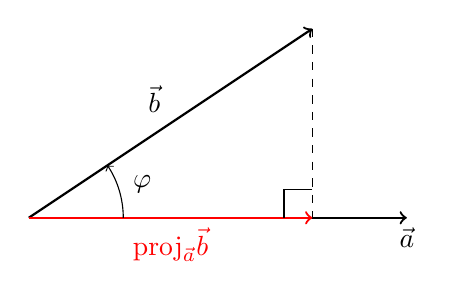
\begin{tikzpicture}[scale=1.2]
    % točke
    \coordinate (O) at (0,0);
    \coordinate (A) at (4,0);      % vektor a (vodoravno)
    \coordinate (B) at (3,2);      % vektor b
    \coordinate (P) at (3,0);      % projekcija B na a
    % osi vektorjev
    \draw[->, thick] (O) -- (A) node[right, below] {$\vec a$};
    \draw[->, thick] (O) -- (B) node[midway, above left] {$\vec b$};
    % projekcija (črtkano)
    \draw[dashed] (B) -- (P);
    % projekcija na a
    \draw[->, thick, red] (O) -- (P) node[midway, below] {$\mathrm{proj}_{\vec a}\vec b$};
    % pravi kot
    \draw (P) ++(-0.3,0) -- ++(0,0.3) -- ++(0.3,0);
    % kot fi
    \draw[->] (1,0) arc (0:34:1);
    \node at (1.2,0.35) {$\varphi$};
\end{tikzpicture}
\end{center}
Z znanjem kotnih funkcij dobimo: $\cos\phi=\frac{\mathrm{proj}_{\vec a}\vec b}{|\vec{b}|}$. Če to vstavimo v osnovno enačbo za skalarni produkt dobimo:
$$\vec{a}\cdot\vec{b}=|\vec{a}|\cdot\mathrm{proj}_{\vec a}\vec b$$
%%%%%%%%%%%%%%%%%%%%%%%%%%%%%%%%%%%%%%%%%%%%%%%%%%%%%%%%%%%%%%%%%%%%%%%%%%%%%%%%%%%%%%%%%%%%%%%%%%%%%%%%%%%%%%%%%%%%%%%%%%%%%%%%%%%%%%%%%%%%%%%%%%%%%%%%%%%%%%%%%%%%%%%%%%%%%%%%%%%%%%%%%%%%%%%%%%%%%%%%%%
\newpage
\section{11. ura: Vaje: Skalarni produkt}
\begin{tabularx}{\textwidth}{|>{\bfseries\RaggedRight}p{2.7cm}|X|}
\hline
Oblika & Vaje pred tablo \\ \hline
Pripomočki & Tabla, kreda \\ \hline
Učni cilji & Samostojno računajo kot med vektorjema in skalarni produkt vektorjev \\ \hline
Predznanje & Znanje prejšnje ure \\ \hline

\end{tabularx}
\\

Ura je namenjena reševanju vaj o skalarnem produktu. 
%%%%%%%%%%%%%%%%%%%%%%%%%%%%%%%%%%%%%%%%%%%%%%%%%%%%%%%%%%%%%%%%%%%%%%%%%%%%%%%%%%%%%%%%%%%%%%%%%%%%%%%%%%%%%%%%%%%%%%%%%%%%%%%%%%%%%%%%%%%%%%%%%%%%%%%%%%%%%%%%%%%%%%%%%%%%%%%%%%%%%%%%%%%%%%%%%%%%%%%%%%
\newpage
\section{12. ura: Izpeljava kosinusnega izreka}
\begin{tabularx}{\textwidth}{|>{\bfseries\RaggedRight}p{2.7cm}|X|}
\hline
Oblika & Frontalna \\ \hline
Pripomočki & Tabla, kreda \\ \hline
Učni cilji & Znajo zapisati in uporabiti kosinusni izrek \\ \hline
Predznanje & Skalarni produkt\\ \hline

\end{tabularx}
\\

Izpeljemo kosinusni izrek. Najprej narišemo nek raznostranični trikotnik ter označimo njegova oglišča, stranice in kote. Stranici $b$ in $c$ označimo z vektorjema $\vec{b}$ in $\vec{c}$, ki imata skupno izhodišče.
Zanima nas, kaj se zgodi, če izračunamo $a^2$: $$a^2=a\cdot a=\vec{BC}\cdot \vec{BC}=(\vec{b}-\vec{c})\cdot (\vec{b}-\vec{c})= |\vec{b}|^2-2\vec{b}\vec{c}+|\vec{c}|^2=b^2+c^2-2|\vec{b}|\cdot|\vec{c}|\cdot\cos\alpha$$
Dobili smo torej: $$a^2=b^2+c^2-2bc\cdot\cos\alpha$$
Podobno bi lahko izpeljali še: $$b^2=a^2+c^2-2ac\cdot\cos\beta$$
$$c^2=a^2+b^2-2ab\cdot\cos\gamma$$
Kosinusni izrek velja za vse trikotnike. Preizkusimo, kaj se zgodi, če ga uporabimo na pravokotnem trikotniku (dobimo Pitagorov izrek).
Povejmo še, kdaj ga lahko uporabimo:
\begin{enumerate}
    \item ko poznamo 2 stranici in vmesni kot (in želimo izračunati tretjo stranico)
    \item ko poznamo vse tri stranice (in želimo izračunati notranji kot)
\end{enumerate}
Sledijo naloge, v katerih uporabljamo kosinusni izrek. Naloge naj ne vključujejo samo izključno trikotnikov, temveč tudi ostale geometrijske like 
(npr. paralelogram, v katerem poznamo dolžine stranic ter en notranji kot ter računamo dolžini obeh diagonal).


%%%%%%%%%%%%%%%%%%%%%%%%%%%%%%%%%%%%%%%%%%%%%%%%%%%%%%%%%%%%%%%%%%%%%%%%%%%%%%%%%%%%%%%%%%%%%%%%%%%%%%%%%%%%%%%%%%%%%%%%%%%%%%%%%%%%%%%%%%%%%%%%%%%%%%%%%%%%%%%%%%%%%%%%%%%%%%%%%%%%%%%%%%%%%%%%%%%%%%%%%%
\newpage
\section{13. ura: Dodatna ura }
\begin{tabularx}{\textwidth}{|>{\bfseries\RaggedRight}p{2.7cm}|X|}
\hline
Oblika &  \\ \hline
Pripomočki &  \\ \hline
Učni cilji &  \\ \hline
Predznanje & \\ \hline

\end{tabularx}
\\

\begin{komentar}
    Morda se nam zdi, da lahko vso to snov z dijaki zelo hitro predelamo, vendar je treba upoštevati da dijaki porabijo veliko časa za prepisovanje snovi s table. Ta dodatna ura je namenjena predvsem rezervi, če nam zmanjka časa v prejšnjih urah.
\end{komentar}
%%%%%%%%%%%%%%%%%%%%%%%%%%%%%%%%%%%%%%%%%%%%%%%%%%%%%%%%%%%%%%%%%%%%%%%%%%%%%%%%%%%%%%%%%%%%%%%%%%%%%%%%%%%%%%%%%%%%%%%%%%%%%%%%%%%%%%%%%%%%%%%%%%%%%%%%%%%%%%%%%%%%%%%%%%%%%%%%%%%%%%%%%%%%%%%%%%%%%%%%%%
\newpage
\section{14. ura: Ortogonalna in ortonormirana baza}
\begin{tabularx}{\textwidth}{|>{\bfseries\RaggedRight}p{2.7cm}|X|}
\hline
Oblika & Frontalna \\ \hline
Pripomočki & Tabla, kreda, (avtomobilčki) \\ \hline
Učni cilji & Razumejo pravokotnost v prostoru \\ \hline
Predznanje & Pojem baze, linearne kombinacije\\ \hline

\end{tabularx}
\\

\begin{komentar}
    Dijaki se danes prvič srečajo s temi pojmi. 
\end{komentar}
Najprej ponovimo, kar že vemo o bazi ravnine in prostora: kakšni vektorji in koliko vektorjev ju sestavlja?\\
\begin{ide}
    Razložimo lahko na primeru avtomobilčkov: zadnjič smo imeli dva avtomobilčka, ki sta se vozila po tabli in sta tako lahko skupaj celotno tablo porisala z vektorji. Avtomobilčka sta bila lahko obrnjena kakorkoli, le po isti premici se nista smela voziti. Za ortogonalno bazo zahtevamo, da sta avtomobilčka postavljena na pravokotnih premicah.
\end{ide}
\textbf{DEFINICIJA:} Baza je \textbf{ortogonalna}, če so bazni vektorji paroma pravokotni.
Baza je \textbf{ortonormirana}, če so bazni vektorji paroma pravokotni in enotski.\\
Najprej dana pojma razložim in predstavim na ravnini, nato pa še v prostoru.
Narišem koordinatni sistem v prostoru, Aplikatna os $z$ kaže navzgor. Na oseh označimo enotske vektorje $i,j,k$. 
Ker so med seboj paroma pravokotni in dolgi eno enoto, tvorijo ortonormirano bazo prostora.
\begin{ide}
    Nekaterim učencem si je zelo težko predstavljati stvari v prostoru. V pomoč lahko prinesem kakšno stvar, ki se s pomočjo vakuuma prilepi na gladko podlago (npr. puščica za otroški lok), ter jo prilepim na tablo tako da mi tvori tretjo os koordinatnega sistema v prostoru. 
\end{ide}
Razmislimo, kako bi lahko splošen vektor zapisali v danih bazah: \\
V ravnini: $\vec{v}=k\vec{i}+m\vec{j}$\\
V prostoru: $\vec{v}=k\vec{i}+m\vec{j}+n\vec{k}$\\
Ta zapis smo spoznali že pri linearni kombinaciji vektorjev tako da ni nič novega.
%%%%%%%%%%%%%%%%%%%%%%%%%%%%%%%%%%%%%%%%%%%%%%%%%%%%%%%%%%%%%%%%%%%%%%%%%%%%%%%%%%%%%%%%%%%%%%%%%%%%%%%%%%%%%%%%%%%%%%%%%%%%%%%%%%%%%%%%%%%%%%%%%%%%%%%%%%%%%%%%%%%%%%%%%%%%%%%%%%%%%%%%%%%%%%%%%%%%%%%%%%
\newpage
\section{15. ura: Komponente vektorja}
\begin{tabularx}{\textwidth}{|>{\bfseries\RaggedRight}p{2.7cm}|X|}
\hline
Oblika & Frontalna \\ \hline
Pripomočki & Tabla, kreda \\ \hline
Učni cilji & Računajo z vektorji, zapisanimi po komponentah \\ \hline
Predznanje & Koordinatni sistem \\ \hline

\end{tabularx}
\\

Ponovimo kaj že vemo o točkah v koordinatnem sistemu. Narišem koordinatni sistem in točke v različnih kvadrantih, dijaki pa povedo koordinate točk ter kako naj to zapišem npr. $A(-3,2)$. Zadnji taki točki naj bosta $I(1,0)$ in $J(0,1)$.\\
Naredimo povezavo med točkami v koordinatnem sistemu in vektorji. Zapišem vektorja $\vec{i}=(1,0)$ in $\vec{j}=(0,1)$. Pokomentiram zapis: tukaj gre za vektorje, zato je nad črkami še vedno puščica, pomembna razlika je enačaj. \\
Za vajo vsem točkam iz začetka ure dodelimo vektorje in jih ustrezno zapišemo s pomočjo komponent. Pogledamo tudi, kako bi zapisali s komponentami vektor $\vec{v}=k\vec{i}+m\vec{j}$ iz prejšnje ure. \\
Omenim, da se tem vektorjem, ki smo jih sedaj obravnavali (ki se začnejo v koordinatnem izhodišču) reče \textbf{krajevni vektorji}. Krajevne vektorje označujemo z $\vec{r}_A$\\

Naredimo par primerov računanja s komponentami. V koordinatni sistem narišemo dva krajevna vektorja. Znamo ju sešteti grafično po trikotniškem pravilu. Sedaj poglejmo, kako bi to naredili računsko z uporabo komponent:\\

\noindent $\vec{a}=(a_1,a_2,a_3)= a_1\cdot\vec{i}+a_2\cdot\vec{j}+a_3\cdot\vec{k}$\\
$\vec{b}=(b_1, b_2,b_3)=b_1\cdot\vec{i}+b_2\cdot\vec{j}+b_3\cdot\vec{k}$\\
\begin{align*}
\vec{a}+\vec{b}
    &= a_1\cdot\vec{i}+a_2\cdot\vec{j}+a_3\cdot\vec{k}
      +b_1\cdot\vec{i}+b_2\cdot\vec{j}+b_3\cdot\vec{k} \\
    &= (a_1+b_1)\cdot\vec{i}
      +(a_2+b_2)\cdot\vec{j}
      +(a_3+b_3)\cdot\vec{k}\\
    &=(a_1+b_1,a_2+b_2,a_3+b_3)
\end{align*}
Podobno lahko naredimo za odštevanje.\\
Poglejmo še \textbf{množenje s skalarjem}:
$$n\cdot\vec{a}=n\cdot(a_1,a_2,a_3)=(n\cdot a_1,n\cdot a_2, n\cdot a_3)$$

%%%%%%%%%%%%%%%%%%%%%%%%%%%%%%%%%%%%%%%%%%%%%%%%%%%%%%%%%%%%%%%%%%%%%%%%%%%%%%%%%%%%%%%%%%%%%%%%%%%%%%%%%%%%%%%%%%%%%%%%%%%%%%%%%%%%%%%%%%%%%%%%%%%%%%%%%%%%%%%%%%%%%%%%%%%%%%%%%%%%%%%%%%%%%%%%%%%%%%%%%%
\newpage
\section{16. ura: Komponente vektorja}
\begin{tabularx}{\textwidth}{|>{\bfseries\RaggedRight}p{2.7cm}|X|}
\hline
Oblika & Frontalna \\ \hline
Pripomočki & Tabla, kreda \\ \hline
Učni cilji & Računajo z vektorji, zapisanimi po komponentah \\ \hline
Predznanje & Znanje prejšnje ure\\ \hline
\end{tabularx}
\\

Ponovimo znanje iz prejšnje ure. Nato se vprašamo, kako bi poljuben vektor (ki ni krajevni) zapisali s pomočjo komponent.
\begin{komentar}
    Prvo uro smo govorili o tem, kako so vsi vektorji, ki jih dobimo s translacijo določenega vektorja, enaki vektorji. Med dijaki zna priti do zmede, ko bodo sedaj ugotovili, da ti vektorji nimajo enakih komponent.
\end{komentar}



Narišemo pravokotni koordinatni sistem v prostoru in označimo točki $A$ in $B$. Želimo zapisati vektor $\vec{AB}$ s pomočjo komponent. Narišemo krajevna vektorja $\vec{r}_A$ in $\vec{r}_B$ ter izrazimo vektor $\vec{AB}$ z njima: $\vec{AB}=\vec{r}_B-\vec{r}_A$
Dobljeno formulo utrdimo na računskem primeru tudi z uporabo komponent.\\

Izpeljimo še, kako bi izračunali razpolovišče daljice $AB$ (označimo ga z $S$):
\begin{align*}
\vec{r}_S
    &= \vec{r}_A+\frac{1}{2}\vec{AB} \\
    &= \vec{r}_A+\frac{1}{2}\left(\vec{r}_B-\vec{r}_A\right) \\
    &= \vec{r}_A+\frac{1}{2}\vec{r}_B-\frac{1}{2}\vec{r}_A \\
    &= \frac{1}{2}\vec{r}_A+\frac{1}{2}\vec{r}_B \\
    &= (\frac{1}{2}a_1,\frac{1}{2}a_2,\frac{1}{2}a_3)+(\frac{1}{2}b_1,\frac{1}{2}b_2,\frac{1}{2}b_3)\\
    &= (\frac{a_1+b_1}{2},\frac{a_2+b_2}{2},\frac{a_3+b_3}{2})
\end{align*}
$$\Rightarrow S(\frac{a_1+b_1}{2},\frac{a_2+b_2}{2},\frac{a_3+b_3}{2})$$


\begin{primer}
    Točka $T$ leži na daljici $AB$ v razmerju $|AT|:|TB|=4:1$. Izračunaj koordinate točke $T$, če imaš podane koordinate točk $A(-2,2,6)$ in $B(3,2,-4)$.
\end{primer}
\begin{komentar}
    Rešitev: $T(2,2,-2)$
\end{komentar}

\begin{ide}
    Za uvedbo komponent:
    en dijak je robot, ki se premika po učilnici tako, kot mu drugi ukažejo: dve mizi naprej, tri stole v desno, ena miza nazaj, itd.  Ali se da z različnimi ukazi priti na enak cilj? njegovo premikanje nato zapišemo z vektorji, kjer prva komponenta pove, koliko stolov je šel levo/desno, druga komponenta pa, koliko miz je šel naprej/nazaj.
\end{ide}
\begin{ide}
Lov na zaklad:
    dijaki dobijo ukaze, ki so zapisani kot vektorji. Dijaki se morajo v pravem zaporedju premakniti toliko miz naprej/nazaj in toliko stolov levo/desno kot jim piše na listku. Ko pridejo do konca, je zaklad skrit na listku pod mizo, na katerem piše objasnitev komponent vektorja.
\end{ide}
%%%%%%%%%%%%%%%%%%%%%%%%%%%%%%%%%%%%%%%%%%%%%%%%%%%%%%%%%%%%%%%%%%%%%%%%%%%%%%%%%%%%%%%%%%%%%%%%%%%%%%%%%%%%%%%%%%%%%%%%%%%%%%%%%%%%%%%%%%%%%%%%%%%%%%%%%%%%%%%%%%%%%%%%%%%%%%%%%%%%%%%%%%%%%%%%%%%%%%%%%%

\section{17. ura: Vaja računanja s komponentami}
\begin{tabularx}{\textwidth}{|>{\bfseries\RaggedRight}p{2.7cm}|X|}
\hline
Oblika & Vaje pred tablo\\ \hline
Pripomočki & Tabla, kreda, vaje \\ \hline
Učni cilji & Samostojno rešujejo vaje v povezavi s komponentami vektorjev \\ \hline
Predznanje & Dosedanje znanje o vektorjih \\ \hline

\end{tabularx}
\\

Ura je namenjena vaji računanja s komponentami. Dijaki hodijo pred tablo, kjer rešujejo vaje.
%%%%%%%%%%%%%%%%%%%%%%%%%%%%%%%%%%%%%%%%%%%%%%%%%%%%%%%%%%%%%%%%%%%%%%%%%%%%%%%%%%%%%%%%%%%%%%%%%%%%%%%%%%%%%%%%%%%%%%%%%%%%%%%%%%%%%%%%%%%%%%%%%%%%%%%%%%%%%%%%%%%%%%%%%%%%%%%%%%%%%%%%%%%%%%%%%%%%%%%%%%

%%%%%%%%%%%%%%%%%%%%%%%%%%%%%%%%%%%%%%%%%%%%%%%%%%%%%%%%%%%%%%%%%%%%%%%%%%%%%%%%%%%%%%%%%%%%%%%%%%%%%%%%%%%%%%%%%%%%%%%%%%%%%%%%%%%%%%%%%%%%%%%%%%%%%%%%%%%%%%%%%%%%%%%%%%%%%%%%%%%%%%%%%%%%%%%%%%%%%%%%%%
\newpage
\section{19. ura: Skalarni produkt v koordinatnem sistemu}
\begin{tabularx}{\textwidth}{|>{\bfseries\RaggedRight}p{2.7cm}|X|}
\hline
Oblika & Frontalna \\ \hline
Pripomočki & Tabla, kreda \\ \hline
Učni cilji & Računajo skalarni produkt z uporabo komponent \\ \hline
Predznanje &  Skalarni produkt, računanje s komponentami\\ \hline

\end{tabularx}
\\

Najprej ponovimo kar že vemo o skalarnem produktu. Nato izpeljimo formulo za izračun skalarnega produkta s pomočjo komponent:\\

\noindent $\vec{a}=(a_1, a_2, a_3)= a_1\vec{i}+a_2\vec{j}+a_3\vec{k}$\\
$\vec{b}=(b_1, b_2,b_3)= b_1\vec{i}+b_2\vec{j}+b_3\vec{k}$\\
\begin{align*}
    \vec{a}\cdot\vec{b}
    &=(a_1\vec{i}+a_2\vec{j}+a_3\vec{k})\cdot(b_1\vec{i}+b_2\vec{j}+b_3\vec{k})\\
    &= \text{Zmnožimo vsakega z vsakim.}\\
    &\quad \text{Če upoštevamo, da so si vektorji $\vec{i},\vec{j}$ in $\vec{k}$ paroma pravokotni, dobimo:}\\
    &=a_1\cdot b_1 + a_2\cdot b_2+a_3\cdot b_3
\end{align*}

S podobnim postopkom bi lahko pokazali naslednje:
$$\vec{a}\cdot (\vec{b}+\vec{c})=\vec{a}\cdot \vec{b}+\vec{a}\cdot\vec{c}$$
$$\vec{a}\cdot\vec{a}= |\vec{a}|^2$$
Iz zadnje formule dobimo formulo za izračun dolžine vektorja: 
$$|\vec{a}|=\sqrt{a_1^2+a_2^2+a_3^2}$$
%%%%%%%%%%%%%%%%%%%%%%%%%%%%%%%%%%%%%%%%%%%%%%%%%%%%%%%%%%%%%%%%%%%%%%%%%%%%%%%%%%%%%%%%%%%%%%%%%%%%%%%%%%%%%%%%%%%%%%%%%%%%%%%%%%%%%%%%%%%%%%%%%%%%%%%%%%%%%%%%%%%%%%%%%%%%%%%%%%%%%%%%%%%%%%%%%%%%%%%%%%
\newpage
\section{20. ura: Vaje -- skalarni produkt v koordinatnem sistemu}
\begin{tabularx}{\textwidth}{|>{\bfseries\RaggedRight}p{2.7cm}|X|}
\hline
Oblika & Vaje pred tablo \\ \hline
Pripomočki & Tabla, kreda \\ \hline
Učni cilji & Usvojijo računanje skalarnega produkta \\ \hline
Predznanje & Dosedanje znanje o vektorjih \\ \hline

\end{tabularx}
\\

Ura je namenjena reševanju vaj iz snovi prejšnje ure. Učenci primere rešujejo na tabli.
\begin{primer}
    Izračunaj realno število $k$, da bo dolžina vektorja $\vec{a}=(k+2,4-2k,3k-1)$ enaka $\sqrt{17}$.
\end{primer}
\begin{komentar}
    Rešitev: $k_1 = 1, k_2= \frac{2}{7}$
\end{komentar}
\begin{primer}
    Določi $y$, da bosta vektorja $\vec{a}=(3,y,-2)$ in $\vec{b}=(-2,-1,-4)$ pravokotna. 
\end{primer}
\begin{komentar}
    Rešitev: $y=2$
\end{komentar}
\begin{primer}
    Dana sta vektorja $\vec{a}=(2x,2,3)$ in $\vec{b}=(-6,-2,-x)$.
    \begin{enumerate}
        \item Določi $x$, da bo dolžina vektorja $\vec{a}$ enaka dolžini vektorja $\vec{b}$.
        \item Določi $x$, da bosta dana vektorja pravokotna.
        \item Določi $x$, da bosta dana vektorja kolinearna.
    \end{enumerate}
\end{primer}
\begin{komentar}
    Rešitev:
    \begin{enumerate}
        \item $x=\pm 3$
        \item $x=-\frac{4}{15}$
        \item $k=-1, x=3$
    \end{enumerate}
\end{komentar}
%%%%%%%%%%%%%%%%%%%%%%%%%%%%%%%%%%%%%%%%%%%%%%%%%%%%%%%%%%%%%%%%%%%%%%%%%%%%%%%%%%%%%%%%%%%%%%%%%%%%%%%%%%%%%%%%%%%%%%%%%%%%%%%%%%%%%%%%%%%%%%%%%%%%%%%%%%%%%%%%%%%%%%%%%%%%%%%%%%%%%%%%%%%%%%%%%%%%%%%%%%
\newpage
\section{21. ura: Vaje }
\begin{tabularx}{\textwidth}{|>{\bfseries\RaggedRight}p{2.7cm}|X|}
\hline
Oblika & Vaje pred tablo \\ \hline
Pripomočki & Tabla, kreda \\ \hline
Učni cilji & Usvojijo računanje z vektorji na grafičnem in računskem nivoju \\ \hline
Predznanje & Dosedanje znanje o vektorjih \\ \hline

\end{tabularx}
\\

Dijaki pred tablo rešujejo vaje, ki se navezujejo na računanje skalarnega produkta v ortonormirani bazi.
%%%%%%%%%%%%%%%%%%%%%%%%%%%%%%%%%%%%%%%%%%%%%%%%%%%%%%%%%%%%%%%%%%%%%%%%%%%%%%%%%%%%%%%%%%%%%%%%%%%%%%%%%%%%%%%%%%%%%%%%%%%%%%%%%%%%%%%%%%%%%%%%%%%%%%%%%%%%%%%%%%%%%%%%%%%%%%%%%%%%%%%%%%%%%%%%%%%%%%%%%%
\end{document}